\documentclass[11pt]{article}

\usepackage{thumbpdf, amssymb, amsmath, amsthm, microtype,
	    graphicx, verbatim, listings, color, fancybox}
\usepackage[pdftex]{hyperref}
%\usepackage[margin=1in]{geometry}
\usepackage{cawsty}
\usepackage{fullpage}
\usepackage{pseudocode}

\usepackage{algorithm}
%\usepackage{algorithmic}
\usepackage{amsmath}
\usepackage{amsthm}
\usepackage{algpseudocode}
\usepackage{algorithmicx}% http://ctan.org/pkg/algorithmicx
\usepackage{lipsum}% http://ctan.org/pkg/lipsum
\usepackage{xifthen}% http://ctan.org/pkg/xifthen
\usepackage{needspace}% http://ctan.org/pkg/needspace
\usepackage{hyperref}% http://ctan.org/pkg/hyperref

% ================ ALGORITHM ENVIRONMENT ================
\newcounter{numberedAlg}% Algorithm counter
\newenvironment{numberedAlg}[1][]%
  {% \begin{numberedAlg}[#1]
    \needspace{2\baselineskip}% At least 2\baselineskip required, otherwise break
    \noindent \rule{\linewidth}{1pt} \endgraf% Top rule
    \refstepcounter{numberedAlg}% For correct reference of algorithm
    \centering \textsc{Algorithm}~\thenumberedAlg%
    \ifthenelse{\isempty{#1}}{}{:\ #1}% Typeset name (if provided)
  }{% \end{numberedAlg}
  \noindent \rule{\linewidth}{1pt}% Bottom rule
  }%

%\setlength{\parindent}{0pt}

\linespread{1.2}

\begin{document}
\arltitle{Trends in Network Robustness Research}{4005-700 Data Communication and Networks I}

\begin{abstract}
Due to the growing pervasiveness of civilian and 
military networks for the transmission of safety-critical and real-time data, 
it is critically important that they are resistant to selective and random network 
node deletions. Network robustness is a measure of the performance and 
throughput responsiveness of a network in response to such deletions. The nature of 
this metrics lends itself to the application of percolation theory, which can be
used to describe the behavior of connected clusters in a random graph. This theory
can be utilized to design and construct optimally robust networks in order to yield
the best performance in the event of node deletions.

This paper presents some background information on network robustness and
its importance in modern communication systems, presents some recent advances
made in the topic, and concludes with avenues of future work that can be explored
by researchers in the field. 
\end{abstract}

% http://crpit.com/confpapers/CRPITV26Dekker.pdf
% http://en.wikipedia.org/wiki/Percolation_theory
% http://arxiv.org/abs/cond-mat/0007300
% http://www.research.ibm.com/people/r/rish/papers/PhysicaA_3_30.pdf
% http://www.cs.berkeley.edu/~dawnsong/papers/coloring_ndss08_cr.pdf

% robust routing and dynamic load balancing - the hw/sw solution to help deal with robustness and traffic changes
% http://iie.fing.edu.uy/investigacion/grupos/artes/publicaciones/casas_drcn09.pdf

\section{Introduction}

Military and civilian communications have seen two common trends in rencent years: an 
increase in network-oriented operations and an increase in high-risk threats to
such networks \cite{Bernard_networkrobustness}. These operational efforts place
high reliance on the underlying network infrastructure for communication, so it is vital
that this communication medium is protected against emerging attacks that focus on
specific nodes in the network or communication lines that join nodes together. In this context
the type of network attacks are irrelevant; the focus is more aligned with the optimal topology
of networks and technological aids that can be utilized to help handle any changes in this topology. 

This focus can be seen by a significant increase in research oriented around robust network design that provides high throughput and connectivitiy among all nodes in the network, especially when specific nodes are intentionally or unintentionally deleted from the network. Subsequently, the robustness of such networks can be viewed as a qualitative or quantitative measure of the network's resilience to such topology changes.

The problem of designing such networks has lent itself as a useful application of both graph theory and percolation theory. Graph theory has been applied to mathematically analyze the robustness of networks represented as undirected graphs based on their levels of vertex and edge connectivity. Similarly, percolation theory has been applied to study the behavior of connected clusters in undirected network graphs. 

This paper will focus on recent research efforts centered around both of these branches of 
mathematical theory and their application to network design. It will also present practical methods of
network engineering that have been employed to help networks deal with topology changes dynamically.
Lastly, it will discuss avenues for future research and open problems that have been posed by 
researchers in the field.

\section{Network Functionality}

It is natural to model any communication network as an undirected graph $G$, which has a fixed 
set of vertices (nodes) $V(G)$ and edges (links) $E(G)$ that represent physical connections between such vertices. The topology of a network
can thus be visualized graphically using elements from these two sets. For the remainder of this paper,
we use the term vertex as a synonom for node and edge as a synonom for communication link. As an example of a graph representing a network, consider a completely connected network with $n$ nodes in which every node can directly communicate with every other 
node can be seen as $K_{n}$, the complete graph on $n$ vertices (that is, $|V(G)|$ $= n$). In such a network, every node $v$ can
communicate with exactly $n-1$ other nodes, which means that its degree $deg(v) = n-1$. 

In order to discuss the connectivity of networks, it is necessary to define the connectivity of such
graphs in terms of both the vertices and edges. We introduce the following terms to use throughout 
the remainder of this paper.

% graph connectivity
\begin{define}
A graph $G$ is said to be \textbf{connected} if and only if $\forall u,v \in V(G)$ there exists a path between $u$ and $v$.
\end{define}

% vertex connectivity
% edge connectivity

The process of measuring the functionality of a network 

\section{Network Attacks}
%HDA - high degree adaptiveness - onion
% from: http://polymer.bu.edu/~hes/networks/hsmah11.pdf

%more from http://www.ncbi.nlm.nih.gov/pubmed/12059649
%Some other attacks are described in \cite{Attacks}

TODO: describe some common networks here, why they are studied, etc
TODO: depends on type of network (is it ad-hoc or fixed topology?)

\subsection{Attack Strategies}
%TODO: vertex/edge based attacks, degree or betweeness attacks
Attacks on large scale networks are not usually ad-hoc; they are based on a logical and structured strategy for dereasing the connectivity of the network by taking as little action as possible. Clearly, if one was to delete all nodes from a network, then that would yield the maximum decrease in connectivity. However, such attacks are not practical, so these strategies must be considered at a smaller scale.

%TODO: print attack paper, read, and include attack summaries in here

\subsection{Vertex Attacks}
TODO

\subsection{Edge Attacks}
TODO

\section{Network Robustness}
%http://arxiv.org/pdf/1203.2982v1.pdf

Many different measures for network robustness have been proposed in recent years. All of which tend
to use the notion of densely connected components in the corresponding graph. In this section we present
a two unique instances of such measurements, one of which is based entirely on node topology and the other that is based on both nodes and their respective edges, and summarize their accuracy when applied to real networks.

\subsection{Node-based Measurement}
A natural way to think of network robustness is from the perspective of individual nodes, since they are 
usually the primary targets in malicious or non-malicious network attacks. Using this idea, Herrmann et al
defined a concise equation for calculating the robustness of a network based on the size of connected
components in the corresponding graph. Mathematically, this can be defined as follows \cite{Onion}:

%24: http://polymer.bu.edu/~hes/networks/hsmah11.pdf
\begin{eqnarray*}
R_{n} = \frac{1}{n}\sum_{q=\frac{1}{n}}^{1}S(q)
\end{eqnarray*}

In laymen terms, this robustness measurement computes the fractions of nodes in the largest connected cluster $S(q)$ after removing $q$ nodes. This is an intuitive calculation, since the goal of engineering robust networks is to ensure the highest measure of connectivity in the event of any node deletions. Furthermore, it has been mathematically verified to represent the exact amount of nodes that need to be deleted for the network to collapse when targeted by high-degree adaptive attacks, which are a specific class of attacks that attempt to remove highly connected nodes from the network. 

In their study of optimal graph structures that yield the highest resilience to such attacks, Herrmann et al found that most networks will exhibit onion topolgies, meaning that there are distinct layers of nodes that are connected, and that each layer $i$ has more connectivity than its parent layer $i+1$ \cite{Onion}. An example of such a graph is shown in Figure~\ref{fig:Onion}.

\begin{figure}[h!]
	\label{fig:Onion}
	\centering
		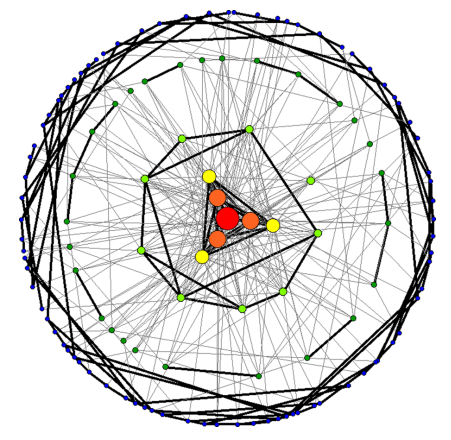
\includegraphics[width=0.5\textwidth]{Onion.jpg}
	\caption{An example of a graph with the onion-like topology \cite{Onion}}
\end{figure}

Herrmann et al have also conducted research on optimization algorithms that increase this robustness measure while at the same time maintaining the distribution of vertex degrees throughout the network. This is an important concept, because their algorithm simply seeks to re-arrange node edges and connections to improve the resilience of the host network to any kinds of attacks. This algorithm can be described as follows:

% the re-structure algorithm
\begin{numberedAlg}[Monte-Carlo-based Robustness Optimization]
\label{alg1}
\begin{algorithmic}[1]
        \item Choose two random edges $(a,b)$ and $(c,d)$ from the graph $G$.
	\item Replace these edges with $(a,c)$ and $(b,d)$.
	\item If $R_{new} > R_{old}$, accept the swap and goto step 1. Otherwise, revert the swap and goto step 1. 
\end{algorithmic}
\end{numberedAlg}

Algorithm~\ref{alg1} is repeated until an ideal level of robustness has been obtained, albiet at the sake of sometimes massive computations (as is the case with Monte-Carlo methods).

\subsection{Node- and Link-based Measurement}
%TODO: http://arxiv.org/pdf/1203.2982v1.pdf

\section{Network Traffic Load}
%TODO: discuss the link load
%TODO: discuss incidents that indicate this importance

\subsection{Dynamic Load Balancing}
%TODO: discuss this technique, with pictures? and examples?

% Here is the bibliography
\bibliographystyle{plain}
\bibliography{nr}

% That's all folks
\end{document}
